\documentclass{ercisbeamer}

\title{Illusions of Knowing}
\subtitle{Effective Studying}
\author{Sven Ligensa}
\institute{European Research Center for Information Systems (ERCIS)}
\date{\today}


\begin{document}

\setbgimage{00_resources/jungle_brain}
\begin{frame}
    \begin{tbox}
        \titlepage
    \end{tbox}
\end{frame}
\setbgimage{}

\begin{frame}{Contents}
    \tableofcontents
\end{frame}

\section{Overview}
\setbgimage{02_resources/feeling_ne_reality}
\begin{frame}{Overview}
    \pause
    \begin{tbox}
        \begin{itemize}
            \item Aka. Illusions of Mastery
            \item Fundamental difference: \red{Feeling $\ne$ Reality}
            \item Everyone is affected, often \negative{not} even \negative{aware}
            \item Fostered by \negative{ineffective learning strategies}
            \item Example of poor metacognition (judgement about what one knows)
            \item \red{Good metacognition}
            \begin{itemize}
                \item Critical for effective decision-making and learning
                \item Skill one must acquire
            \end{itemize}
        \end{itemize}
    \end{tbox}
\end{frame}

\section{Familiarity Trap}
\begin{frame}{Familiarity Trap}
    \begin{tbox}
        \begin{itemize}
            \item Feeling that you know something
            \begin{itemize}
                \item[$\Rightarrow$] No longer need to practice it
                \item[$\Rightarrow$] Bad decisions on what to learn
            \end{itemize}
            
            \item \red{Fluency illusion}: Confuse: Fluency with text $\Leftrightarrow$ Mastery of its content
            \begin{itemize}
                \item \emph{Which learning strategy fosters this illusion? \pause $\rightarrow$ \negative{Rereading}}
            \end{itemize}
        \end{itemize}
    \end{tbox}
\end{frame}

\setbgimage{02_resources/mutable_memory}
\section{Mutable Memory}
\begin{frame}{Mutable Memory}
    \pause
    \begin{tbox}
        \begin{itemize}
            \item Memory = Reconstruction $\ne$ Reality
            \item Two-edged sword
            \begin{itemize}
                \item \negative{Skews our perceptions} \grey{$\Rightarrow$ Stay open to the fallibility of your certainties}
                \item \positive{Essential for learning}
            \end{itemize}
            \item \red{Hindsight Bias}: Tendency to overestimate how much one knew before an event happened $\Rightarrow$ Overconfidence
            \begin{itemize}
                \item \emph{How does it affect our studying? \pause $\rightarrow$ Coming into a tutorial session without working on the exercises beforehand $\Rightarrow$ Feeling that the exercises are easier than they actually are}
            \end{itemize}
            \item \red{Curse of Knowledge}: Tendency to underestimate how much time is needed for another person to learn something new or perform a task
            \begin{itemize}
                \item \emph{Where is this important in the university context? \pause $\rightarrow$ When teaching others, better schedule a bit more time (giving a presentation/tutorial)}
            \end{itemize}
        \end{itemize}     
    \end{tbox}
\end{frame}
\setbgimage{}

\section{Further Illusions}
\begin{frame}{Further Illusions}
    \begin{itemize}
        \item \red{Many} more cognitive biases
        \item \url{https://en.wikipedia.org/wiki/Cognitive_bias}
    \end{itemize}
    \centering
    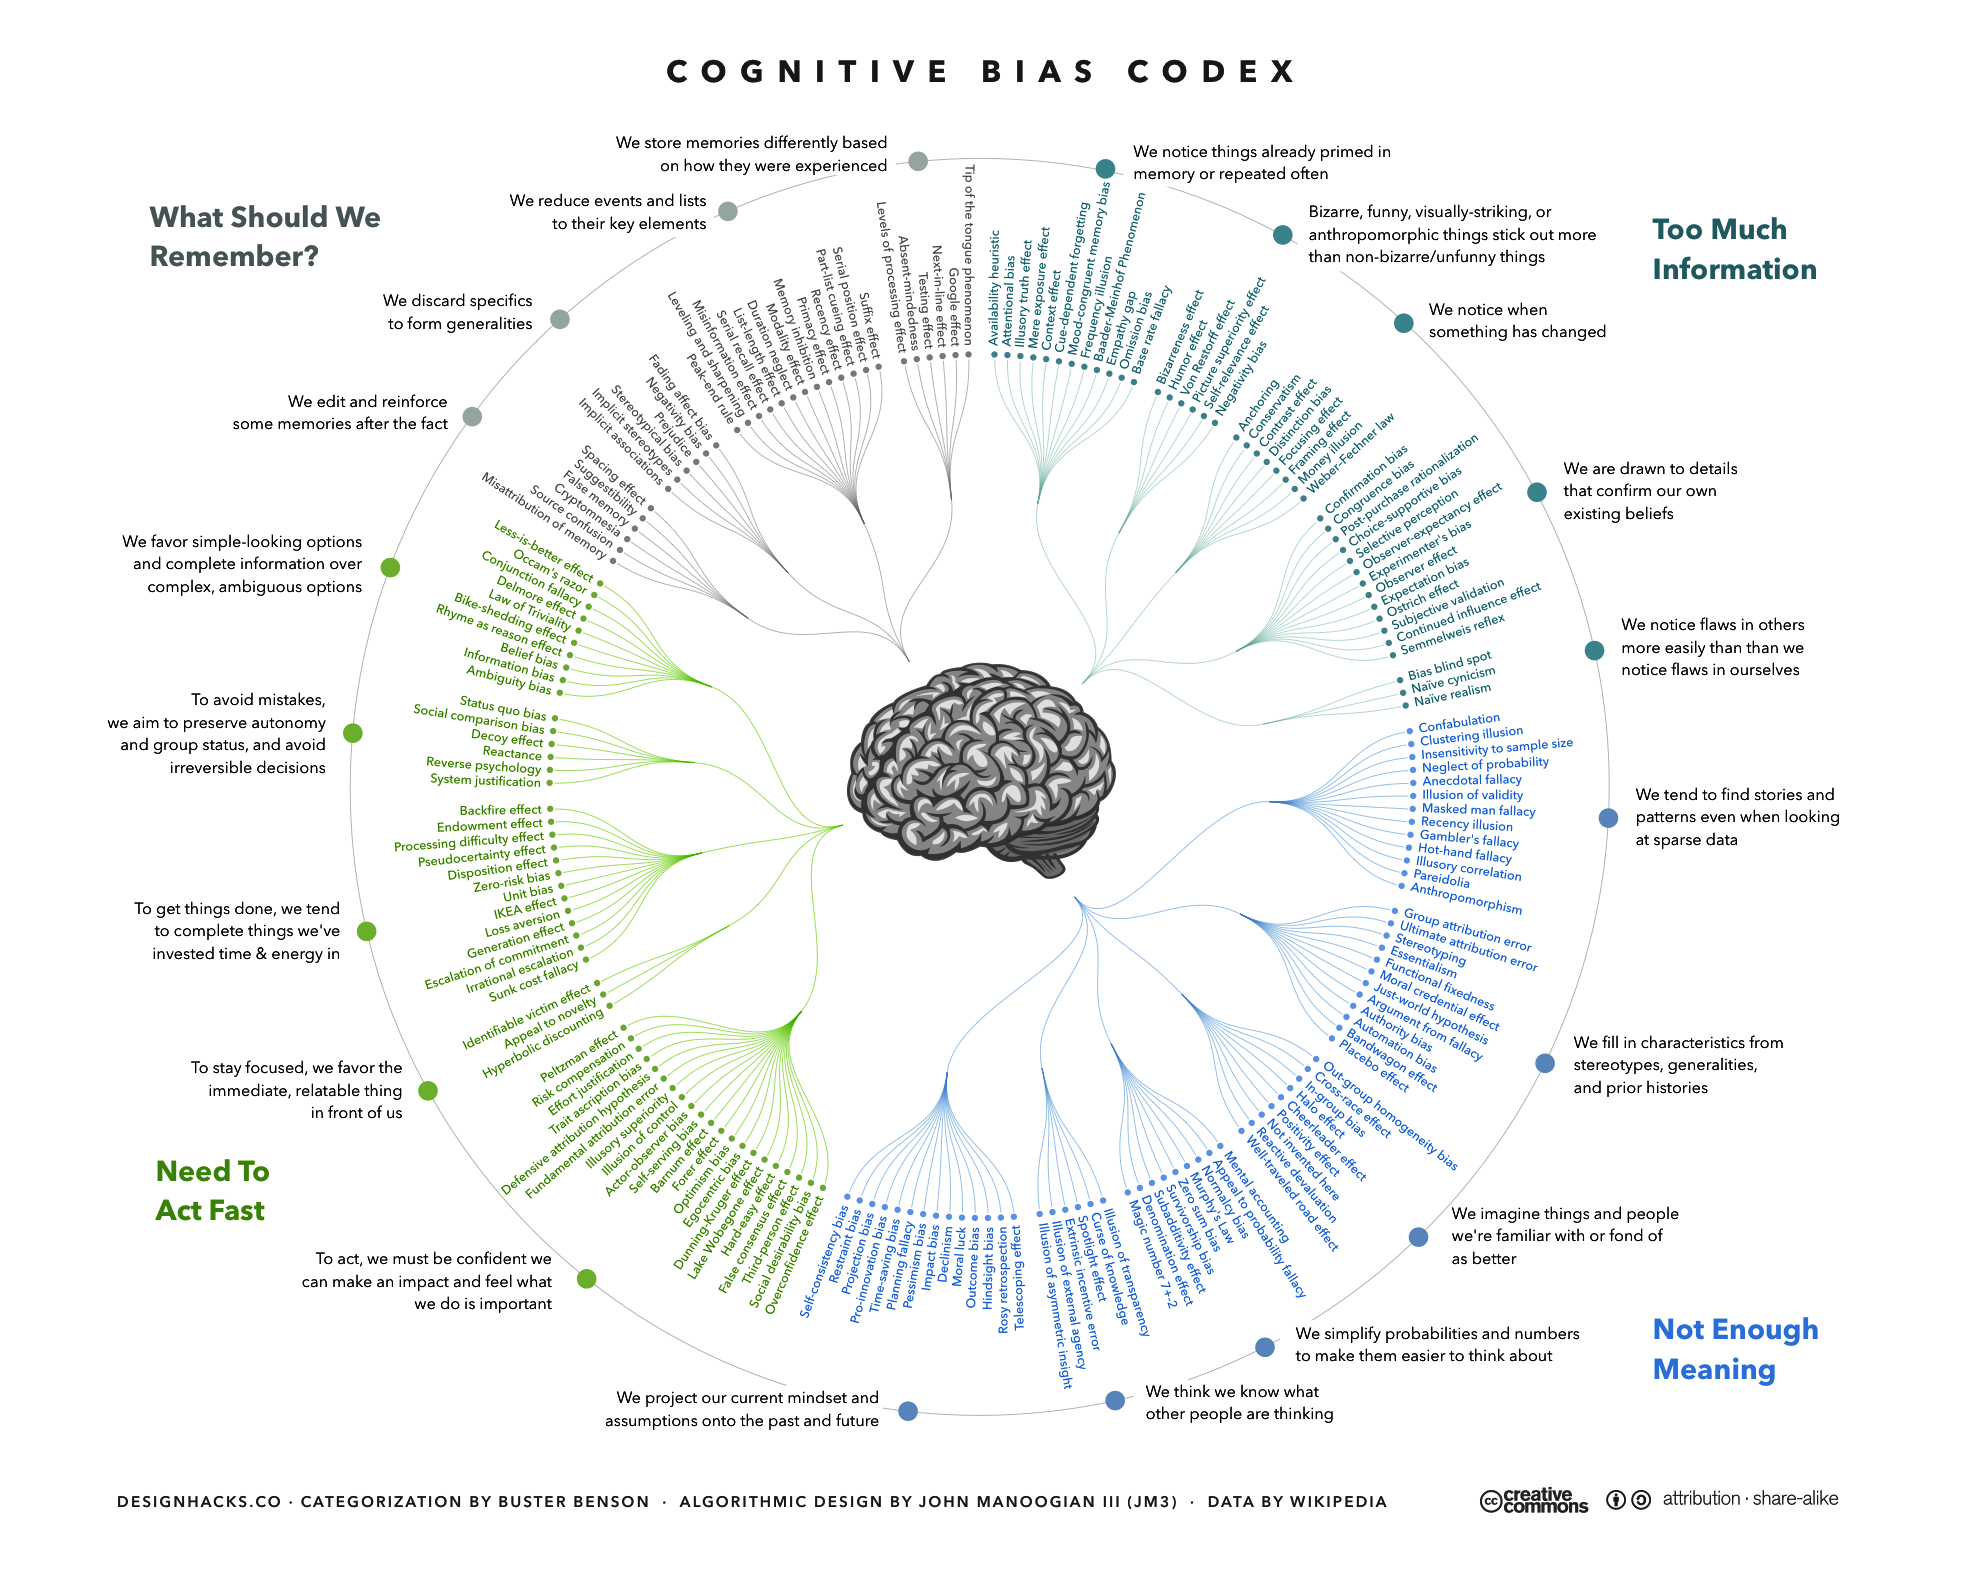
\includegraphics[width=.45\paperwidth]{02_resources/cognitive_bias_codex.png}
\end{frame}

\section{Remedies}
\begin{frame}{Remedies}
    \begin{itemize}
        \item \red{Effective learning strategies} like Retrieval
        \item \red{Objective ways} to track progress
        \item \red{``Practice like you play''}
        \item Practice with \red{others}
        \begin{itemize}
            \item Work alongside more skilled partner
            \item Seek corrective feedback
        \end{itemize}
        \item Be aware of what \red{criteria} you use to judge what you have learned
        \begin{itemize}
            \item \emph{What are good/bad criteria?} \pause
            \begin{itemize}
                \item \emph{\positive{Explaining} a text well using own words}
                \item \emph{\negative{Familiarity} with text}
            \end{itemize}
        \end{itemize}
    \end{itemize}
\end{frame}

\chapteroverview{2}

\thankyou{Happy Learning!}{sven.ligensa@uni-muenster.de}

\sources

\end{document}
